% Fuente vectorial de la figura de arquitectura de conectividad del N150.
% Compilar con: pdflatex conexionN150.tex  (genera conexionN150.pdf)
\documentclass[tikz,border=4pt]{standalone}
\usepackage[T1]{fontenc}
\usepackage[scaled]{helvet}
\renewcommand{\familydefault}{\sfdefault}
\usepackage{fontawesome5}
\usetikzlibrary{arrows.meta,positioning,calc}

\definecolor{n150fill}{HTML}{DAE8FC}
\definecolor{n150line}{HTML}{6C8EBF}
\definecolor{iconblue}{HTML}{1E88E5}
\definecolor{wifiteal}{HTML}{10739E}

\begin{document}
\begin{tikzpicture}[
    font=\small,
    box/.style={draw, fill=white, minimum height=1.25cm, align=center},
    arr/.style={-{Stealth[length=2.2mm]}, thick},
    darr/.style={{Stealth[length=2.2mm]}-{Stealth[length=2.2mm]}, thick},
  ]

  % Contenedor N150
  \draw[n150line, fill=n150fill, line width=1pt, rounded corners=14pt]
    (0,0) rectangle (9.4,6.3);
  \node[font=\bfseries\normalsize] at (4.7,5.9) {N150};

  % Modem
  \node[box, minimum width=3.6cm] (bg95) at (6.3,4.55)
    {\textbf{Quectel BG95}\\[1pt]{\scriptsize (GSM/CAT-M1/NB-IoT)}};
  \node[wifiteal, rotate=45, font=\large] at ($(bg95.north east)+(-0.05,0.18)$) {\faWifi};

  % ESP32
  \node[box, minimum width=3.6cm, minimum height=2.0cm, anchor=north] (esp) at (6.3,2.45) {};
  \node[font=\bfseries] at ($(esp.north)+(0,-0.35)$) {ESP32};
  \node[font=\scriptsize] at ($(esp.north)+(0,-0.75)$) {(MCU + BLE + Wi-Fi)};
  \node[fill=iconblue, text=white, rounded corners=3pt, minimum size=0.65cm, font=\normalsize]
    at ($(esp.south)+(-0.9,0.5)$) {\faWifi};
  \node[fill=iconblue, text=white, rounded corners=3pt, minimum size=0.65cm, font=\normalsize]
    at ($(esp.south)+(0.9,0.5)$) {\faBluetoothB};

  % PIC
  \node[box, minimum width=3.4cm] (pic) at (2.1,1.45)
    {\textbf{PIC24FJ64GU205T}\\[1pt]{\scriptsize (Control del ciclo)}};

  % Conexiones internas
  \draw[arr] ($(esp.north)+(-0.8,0)$) -- ($(bg95.south)+(-0.8,0)$);
  \draw[arr] ($(bg95.south)+(0.8,0)$) -- ($(esp.north)+(0.8,0)$);
  \draw[arr] ([yshift=3mm]pic.east) -- ([yshift=3mm]pic.east -| esp.west);
  \draw[arr] ([yshift=-3mm]pic.east -| esp.west) -- ([yshift=-3mm]pic.east);

  % Comandos AT (sobre las flechas)
  \node[box, minimum width=2.6cm, minimum height=0.55cm, font=\scriptsize] at (6.3,3.0) {Comandos AT};

  % Elementos externos
  \node[font=\fontsize{34}{34}\selectfont] (tower) at (11.3,4.6) {\faBroadcastTower};
  \node[font=\fontsize{30}{30}\selectfont] (phone) at (11.3,1.45) {\faMobile*};
  \node[text=iconblue, font=\fontsize{30}{30}\selectfont] (cloud) at (14.2,3.0) {\faCloud};
  \node[below=0pt of cloud] {Sensify Cloud};

  % Enlaces externos
  \draw[darr] (bg95.east) -- (tower.west);
  \draw[darr] ([yshift=-1.5mm]esp.east) -- ([yshift=-1.5mm]esp.east -| phone.west);
  \draw[darr] ($(tower.south east)+(0.05,0.2)$) -- ($(cloud.north west)+(0.1,-0.1)$);
  \draw[darr] ($(phone.north east)+(0.05,-0.2)$) -- ($(cloud.south west)+(0.1,0.1)$);
\end{tikzpicture}
\end{document}
